\documentclass{article}
\usepackage{amsfonts}
\usepackage{graphicx}
\usepackage{hyperref}
\usepackage{amsmath}
\usepackage{physics}
\usepackage{tikz}
\title{Reaction-Advection-Diffusion Models of Air Pollution}
\author{Daniel Henricks}


\begin{document}

\maketitle

\section{Introduction}

Airborne pollutants are the single most impactful environmental risk to human health, with about one in nine deaths worldwide
attributed to air pollution (Cohen et al., 2017). Poor air quality can cause many negative implications to human health; exposure to
more air pollution is directly correlated to an increased rate of heart attacks and asthma. There are a few different types of air pollution
that can cause adverse affects on human health. First, fine particulate matter ($\text{PM}_{2.5}$) causes approximately 95\% of the deaths due 
to air pollution. ($\text{PM}_{2.5}$) is defined to be any microscopic particles that are of diameter of less than $2.5 \mu$m, about 20 times smaller than the diameter of
a human hair. 

Due to the minute scale of these particles, particulate matter is capable of traveling deep into vital organs such as the lungs or the bloodstream.
Exposure to increased rates of fine particulate matter can lead to coughing and difficulty breathing. Particulate matter is typically produced by the combustion of gasoline, oil, or wood, but has recently
been discovered to occur at smaller rates from natural processes such as volcanic eruptions (Thangavel et al., 2022). In addition to particulate matter, surface-level ozone
($\text{O}_3$) and nitrogen dioxide ($\text{NO}_2$) also contribute to the damages to human health from air pollution. In this paper, we will validate recent diffusion models of 
air pollution and the models to estimate damages to human health caused by pollution.

\section{Types of Models}

Before beginning on the mathematics behind a differential equation model of air pollution, we will discuss how to form a model of air pollution.
One of the main problems with making a diffusion model for air pollution is estimating the flux term of the diffusion equation. We apply Fick's first and second laws of diffusion; 
recall that Fick's first law relates the flux, $J$ to the diffusion constant $k$, and the change in the concentration gradient $c$:

\begin{equation}
    J = -k \* \frac{dc}{dx}
\end{equation}

Typically, chemical transport models (CTMs), programs that simulate and predict atmospheric chemistry, are used to find the fluxes needed in a diffusion equation. 
There are two classes of CTMs: Eulerian and Lagrangian. Eulerian models have an observer standing in one location who is watching the air pass by, 
whereas the Lagrangian models have the observer moving along with the parcel of air as it takes a random walk through the atmosphere (Vallero, 2021).

However, executing CTMs can be computationally difficult. We will first look at a simple model for representing the concentrations of chemicals in the 
atmosphere.

\subsection{A Simple Model}

The model we will first investigate is called the one-box model (Jacob, 1999).

\begin{figure}[h]
   \centering
   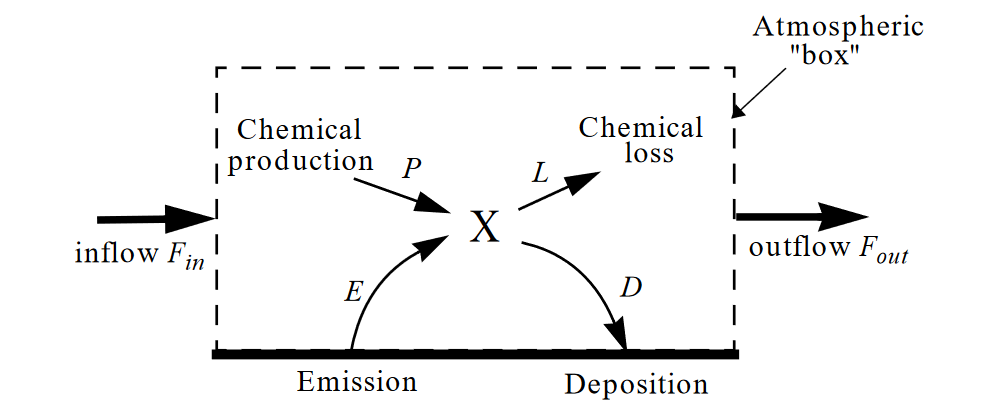
\includegraphics[width=0.8\textwidth]{atmospheric_model.png}
   \caption{One-box model for an atmospheric species X}
   \label{fig:atmospheric_box_model}
\end{figure}

The one-box model for an atmospheric species X is illustrated in Figure~\ref{fig:atmospheric_box_model}. 
The model describes the concentration of X inside of some subset of the global atmosphere (ex: the United States).
The transport rate is described using the flow in, $F_{in}$, and the flow out of, $F_{out}$ of the box. By conservation, the global
atmosphere must obey
$$
    F_{in} = F_{out} = 0
$$
The other parameters of the model are:
\begin{itemize}
   \item Chemical production ($P$)
   \item Emissions ($E$)
   \item Chemical loss ($L$)
   \item Deposition ($D$)
\end{itemize}

We will now define the lifetime, $\tau$, of a molecule, to be the average time a molecule of X remains in our box. 
This will be the mass of the particle divided by the outflow of the box:

\begin{equation}
    \tau = \frac{m}{F_{out}+L+D}    
\end{equation}

We also can set up a mass balance differential equation. The change of the abundance of a species must be equal to the sources less the sinks:

\begin{equation}
    \frac{dm}{dt} = F_{in} + E + P - F_{out} - L - D
\end{equation}

We need to represent the sinks using some loss rate. Let's assume that the losses are proportional to the amount of the species in the box, so the losses are
equal to $km$. (It turns out trivially that $k = \frac{1}{\tau}$). Let's also assume that the sources are independent of $m$ and are 
equal to some constant $S$. Then, we yield the ODE

\begin{equation}
    \frac{dm}{dt} = S - km
\end{equation}

which can be solved quite simply via separation of variables:

$$
    \frac{dm}{dt} = S - km
$$

$$
    \implies \int_0^t \frac{dm}{S-km} = \int_0^t dt
$$

$$
    \implies \frac{-1}{k} \ln{\abs{\frac{S-km(t)}{S-km(0)}}} = t
$$

$$
    \implies S - km(t) = Se^{-kt} - km(0)e^{-kt}
$$

\begin{equation}
    \implies m(t) = \frac{S}{k}(1-e^{-kt}) + m(0)e^{-kt}
\end{equation}

Finding the steady state of this equation yields $S_\infty = \frac{S}{k}$ (via taking the limit as $t \rightarrow \infty$).

This steady state assumption is reasonable because the rate of change of the mass, $\frac{dm}{dt}$, tends to be very small in
comparison to the production rate. Because of this, we classify this steady state as a quasi steady state. 

\subsection{A More Realistic Model: the Puff Model}

We will now investigate a puff model; such a model describes fluid elements moving in space. Note that the puff model
is an example of a Lagrangian model (as mentioned above). We define a fluid element
to be a volume of air in which all particles move with the same velocity. The most common application of a puff model is diffusion from a 
smokestack, something that is essential for understanding how air pollution diffusion. We define the mass balance equation for this model
to be 

\begin{equation}
    \frac{dX_{c}}{dt} = E + P - L - D
\end{equation}

where $X_{c}$ is the concentration of element X. Assume that the puff takes a column shape and that the height of the column is $h$.
Also assume that there is no chemical production ($P$) and that the losses are proportional to the concentration at some rate $L = kX_{c}$. 
We then form the mass-balance equation:

\begin{equation}
    \frac{dX_{c}}{dt} = \frac{E}{h} - kX_{c}
\end{equation}
This is another separable ODE which is trivial to solve. The puff model's steady states are only valid in low-wind conditions, however (Zannetti, 1985).
Many computer systems used by the federal government to predict air pollution use variations of this model with more complicated parameters.

\section{A first diffusion model}

We will first review the diffusion model established by Tirabassi (1989). Analytical models such as this one use solutions to the 
advection-diffusion equation below:

\begin{equation}
    u\frac{\partial C}{\partial x} = \frac{\partial}{\partial y} (K_y \frac{\partial C}{\partial y}) + \frac{\partial}{\partial z} (K_z \frac{\partial C}{\partial z}) + S
\end{equation}

where the parameters are:

\begin{itemize}
    \item Mean wind velocity ($u$)
    \item Concentration ($C$)
    \item Source term ($S$)
    \item Lateral eddy exchange constant ($K_y$)
    \item Vertical eddy exchange constant ($K_z$)
 \end{itemize}
 
This model was further improved by Buske et. al (2012). In this paper, the initial equation was revised to break the concentration
into a three-dimensional problem as seen below:

\begin{equation}
    u\frac{\partial c}{\partial x} + v\frac{\partial c}{\partial y} + w \frac{\partial c}{\partial z} 
    = \frac{\partial}{\partial x} (K_x \frac{\partial c}{\partial x}) + \frac{\partial}{\partial y} (K_y \frac{\partial c}{\partial y}) + \frac{\partial}{\partial z} (K_z \frac{\partial c}{\partial z})
\end{equation}

This equation essentially states that the mean wind vector can be broken up into its components and that the suspended material must be conserved.
We limit the domains of $x$, $y$, and $z$ to $0 < x < L_x$, $0 < y < L_y$, and $0 < z < h$, where $h$ is the height of the atmospheric boundary layer. 
We also impose a value of zero for the eddy diffusivities at the edges of the domain. Since the solution to the three-dimensional problem can be hard to find,
we want to find a way to transform this equation to a two-dimensional problem. To do this, we need to transform the problem to one with variables $x$ and $z$:

First, we create a complete set of orthogonal basis functions in the y-direction over the y-domain. Define

$$
    Y_m(y) = cos(\lambda_m y)
$$
and 
$$
    \lambda_m = \frac{m\pi}{L_y}, m \in \mathbb{N}^{+}
$$

From doing this, we have created a way for any function $f(y)$ to be represented as some linear combination of these eigenfunctions:

$$
    f(y) = \sum_{m=0}^{\infty} c_m Y_m(y)
$$

We then plug in our unknown coefficient of two variables to get equation (4) in Buske (2012):

\begin{equation}
    f(y) = \sum_{m=0}^{\infty} c_m(x, z) Y_m(y)
\end{equation}

To find the value of this coefficient, we will first define some integrals. Let $Y_n(y)$ also be a orthogonal eigenfunction. Then we define

$$
    \int_0^{L_y} Y_m(y)Y_n(y) dy = \alpha_{mn}
$$

$$
    \int_0^{L_y} Y_m'(y)Y_n(y) dy = \beta_{mn}
$$

$$
    \int_0^{L_y} K_y Y_m(y)Y_n(y) dy = \gamma_{mn}
$$

$$
    \int_0^{L_y} K'_y Y'_m(y)Y_n(y) dy = \eta_{mn}
$$

This will help simplify our derivation for finding the unknown constant $c_m(x, z)$.

We first take the chain rule of each of the terms in the diffusion equation and plug in our new equation for the concentration:
$$
    \frac{\partial}{\partial x} [K_x \frac{\partial c(x, y, z)}{\partial x}] = [\frac{\partial}{\partial x} (K_x \frac{\partial c(x, z)}{\partial x}) + K_x \frac{\partial^2 c(x, z)}{\partial x^2}]Y_m(y)
$$

The same process is done for the y-derivative, yielding

$$
    K_y' c_m(x, z) Y_m'(y) + K_y \frac{\partial^2 c}{\partial y^2} c_m(x, z) \cos(\lambda_m y)
$$

The z-derivative also follows the same process, which will be omitted for brevity. To put the equations into the form specified above, we evaluate 
the derivatives and then move over the advection terms. Doing this yields, as shown briefly above,

$$
    [\frac{\partial}{\partial x} [K_x \frac{\partial c(x, z)}{\partial x}] + \frac{\partial}{\partial z} [K_z \frac{\partial c(x, z)}{\partial z}] - u \frac{\partial c(x, z)}{\partial x} - w \frac{\partial c(x, z)}{\partial z}] Y_m(y)
$$

The rest of the terms in the equation come from the chain rule affects of the y derivative. The first term can be reorganized as

$$
    c_m(x, z) K_y' Y_m'(y)
$$

and the second term as 

$$
    c_m(x, z) K_y Y_m''(y)
$$

where 

$$
    Y_m''(y) = -\lambda_m^2 \cos(\lambda_m y) = -\lambda_m^2 Y_m(y)
$$

Substituting, we get 

$$
    -\lambda_m^2 c_m(x, z) K_y Y_m(y)
$$

We have now completed most of the tedious algebra. We then can apply the operator $\int_0^{L_y} Y_n(y) dy$ to obtain the result


\begin{equation}
\begin{aligned}
    \sum_{m=0}^{\infty} \Bigg[ &\frac{\partial}{\partial x} \left( K_x \frac{\partial c(x, z)}{\partial x} \right) + \frac{\partial}{\partial z} \left( K_z \frac{\partial c(x, z)}{\partial z} \right) \\
    &- u \frac{\partial c(x, z)}{\partial x} - w \frac{\partial c(x, z)}{\partial z}  \alpha_{mn} \\
    &- v c_m(x, z) \beta_{mn} \\
    &- \lambda_m^2 c_m(x, z) \gamma_{mn} \\
    &+ c_m(x, z) \eta_{mn} \Bigg]
\end{aligned}
\end{equation}

We now will make some assumptions to simplify this equation. In the ABL, it is common to treat the speeds $v$ and $w$ as zero, such as in Tirabassi (1989).
We also assume that the force of advection is much more dominant than the force of diffusion in the x-direction. Mathematically, this is

$$
    u \frac{\partial c(x, z)}{\partial x} \gg \frac{\partial}{\partial x} (K_x\frac{\partial c(x, z)}{\partial x})
$$

Because of this, we can neglect the diffusion component $K_x$. We also consider that $K_y$ only depends on the z-direction.

We can now rewrite equation (11) above as:

\begin{equation}
    u \frac{\partial c(x, z)}{\partial x} = \frac{\partial} {\partial z} (K_z \frac{\partial c(x, z)}{\partial z}) - \lambda_m^2 K_y c_m(x, z)
\end{equation}

\subsection{An interpretation of this result}

This result turned out to be very accurate against experimental data (Buske, 2012). 
The equation shown above was ran against data from Copenhagen, Denmark, and Kinkaid, Illinois. 
The difference between the predicted and actual results turned out to be within an appropriate 
error bound, leading for the authors to conclude that analytical solutions to the advection differential
equation (ADE) may be possible. The potential for creating an accurate and computationally efficient model
for modeling air pollution dispersion encouraged more research into new methods of CTMs.

\section{InMAP: A more computationally efficient model for finding emissions}

One of the recent developments in the study of air pollution was the creation of computationally efficient models for computing the harm to human health from
diffusion. A prevalent model that has been implemented in industry by companies such as WattTime is InMAP \url{(http://spatialmodel.com/)}. 
InMAP is a model that evaluates pollution by simplifying typical CTMs via using an annual-average basis for its results. InMAP itself
was based on a revolutionary CTM, WRF-Chem (Grell et al., 2005). 

\subsection{How does WRF-Chem work?}

WRF-Chem is a CTM that is based on the Weather Research and Forecasting Model (WRF). The WRF was initially created by
researchers in the late 1990s via a collaboration between the National Center for Atmospheric Research (NCAR), 
the National Oceanic and Atmospheric Administration, and many others. WRF is most useful for its capability to 
apply a mathematical model via a direct simulation with idealized conditions or use actual atmospheric data.
It is used at many meterological companies as well as in solar companies, laboratories, and many other locations.

\begin{figure}[h]
    \centering
    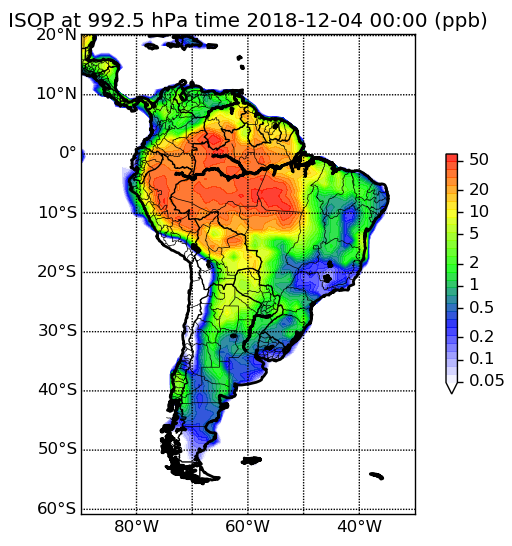
\includegraphics[width=0.3\textwidth]{wrfchem.png}
    \caption{An example of the graphics produced by WRF Chem.}
    \label{fig:atmospheric_box_model}
 \end{figure}

WRF-Chem combines this with the ability to trace $PM_{2.5}$. It is very numerically consistent and its forecasts are 
stronger than many models beforehand. However, like many other CTMs, WRF-Chem is very computationally expensive. 

\subsection{InMAP's solutions}

To solve many of the computational issues that WRF-Chem had, InMAP makes several key simplifications. InMAP simplifies many of the 
marginal emissions rates into annual averages, creating an algorithm that can be run much more efficiently. In addition to being more
computationally efficient, InMAP also creates more spatially detailed results. This efficiency is achieved by using a variable-resolution grid:
areas with a higher density of people are modeled with a higher spacial detail than regions of lower density. The algorithm is able to be downloaded
and is programmed using the Go programming language; it is designed to be simple enough for a beginner user to learn. The authors claim that this is a
novel approach to CTMs.

\begin{figure}[h]
    \centering
    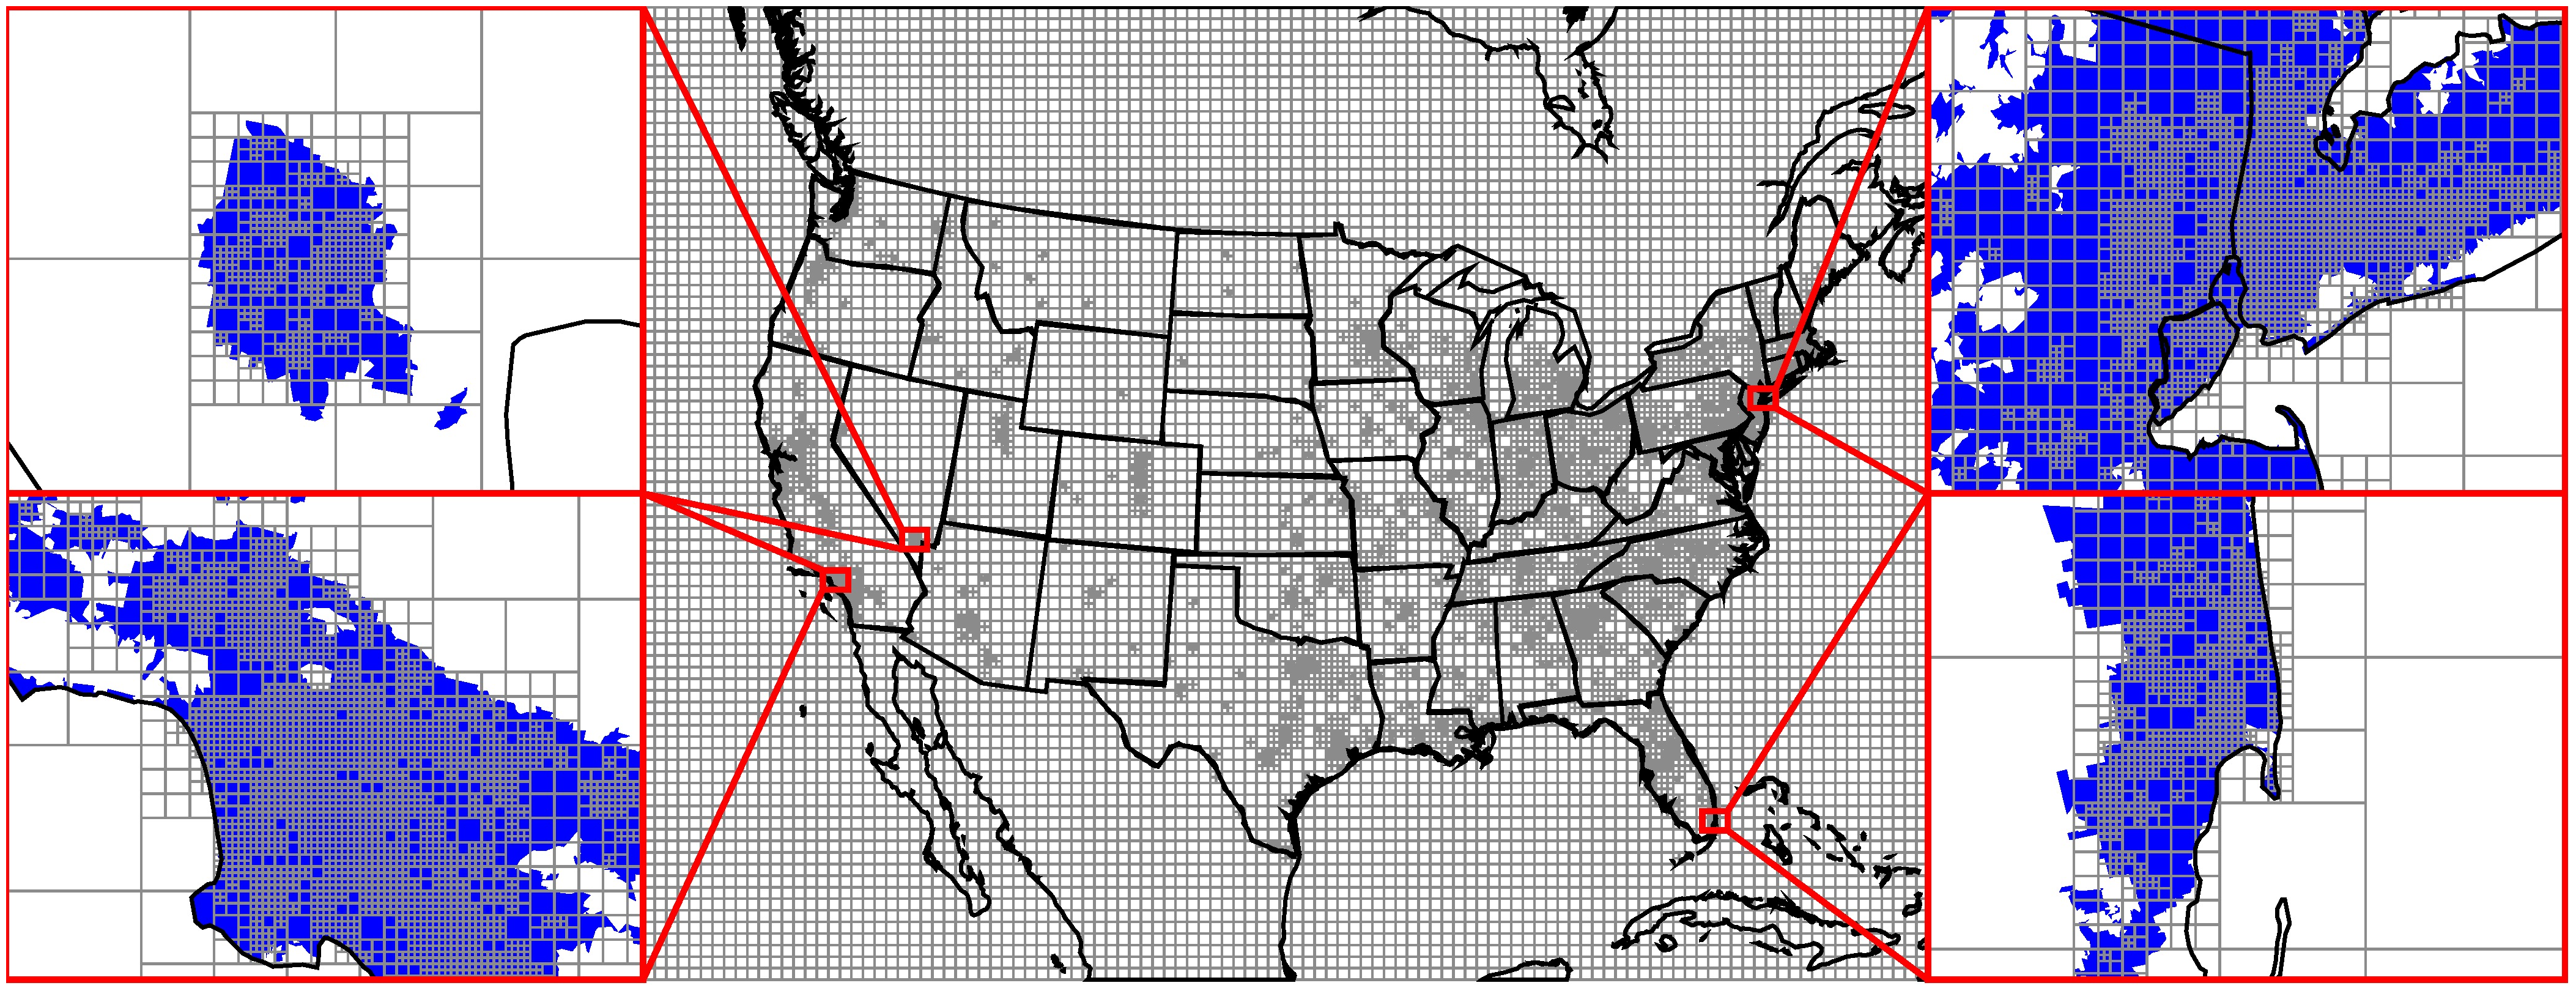
\includegraphics[width=\textwidth]{inmap.png}
    \caption{How InMAP splits the US into regions. Note how regions with higher population density are modeled as smaller grid
    regions, and regions with lower density have larger grid regions}
    \label{fig:grid}
 \end{figure}

\subsection{The diffusion equation}

InMAP utilizes a reaction-advection-diffusion equation to find its air pollution concentrations:

\begin{equation}
    \frac{\partial C_i}{\partial t} = \underbrace{\nabla \cdot (D\nabla C_i)}_{\text{Diffusion Term}} - \underbrace{\nabla \cdot (\vec{v}C_i)}_{\text{Advection Term}} + \underbrace{\sum_{j=1}^{n} R_{ij}}_{\text{Reaction Terms}} + \underbrace{E_i}_{\text{Source/Sink Term}} - \underbrace{d_i}_{\text{Decay Term}}
\end{equation}
    
where 

\begin{itemize}
    \item $C_i$ is the concentration of one of $n$ model pollutant species.
    \item $D$ is a molecular diffusion coefficient (neglected here as a negligible source of chemical transport in the atmosphere compared to advection).
    \item $\vec{v}$ is the wind vector.
    \item $R_{ij}$ is the net formation rate of species $i$ from species $j$.
    \item $E_i$ is pollutant emission.
    \item $d_i$ is pollutant removal via wet and dry deposition.
\end{itemize}

InMAP solves this equation for the concentrations of $\text{PM}_{2.5}$ and many other harmful chemicals emitted. To find the concentrations,
InMAP runs in each grid region at a discrete step interval. During each step, the following are performed: 

\begin{enumerate}
    \item InMAP finds the flux that comes from new emissions. This is done using the plume model, as referenced before. 
    \item The algorithm then calculates how changes in pollutant concentrations are affected by physical and chemical processes including advection, turbulent mixing, etc.
    \item Each process listed above uses a snapshot of the concentration before the time step had occurred to avoid combining changes to concentrations at the same time. 
  \end{enumerate} 

\subsection{How InMAP takes in data}

InMAP first takes in the data and runs it through a preprocessor that is an extension of WRF-Chem. This reduces the complexity of the operations
that need to be ran after. Since the CTM is computationally expensive to run, the input data time step is once per WRF-Chem simulation hour. 
After this, the InMAP algorithm runs stepwise, adjusting the relevant terms of the equation as needed. One of the more interesting features is the 
methodology of updating the advection wind vectors. The wind speed updates at too fast of a rate for any computer to calculate using discrete steps.
To solve this problem, Reynolds decomposition is used: this is a mathematical technique that uses the expected value
of a wind stream and its deviations to calculate an accurate result. For example, if a variable $x$ is decomposed, it would be 
represented as the following equation: 

\begin{equation}
    x = \overline{x} + x'
\end{equation}

where

\begin{itemize}
    \item $\overline{x}$ is the expected value of $x$
    \item $x'$ is deviations in x.
\end{itemize}

An example of the output of the algorithm is shown below:


\begin{figure}[h]
    \centering
    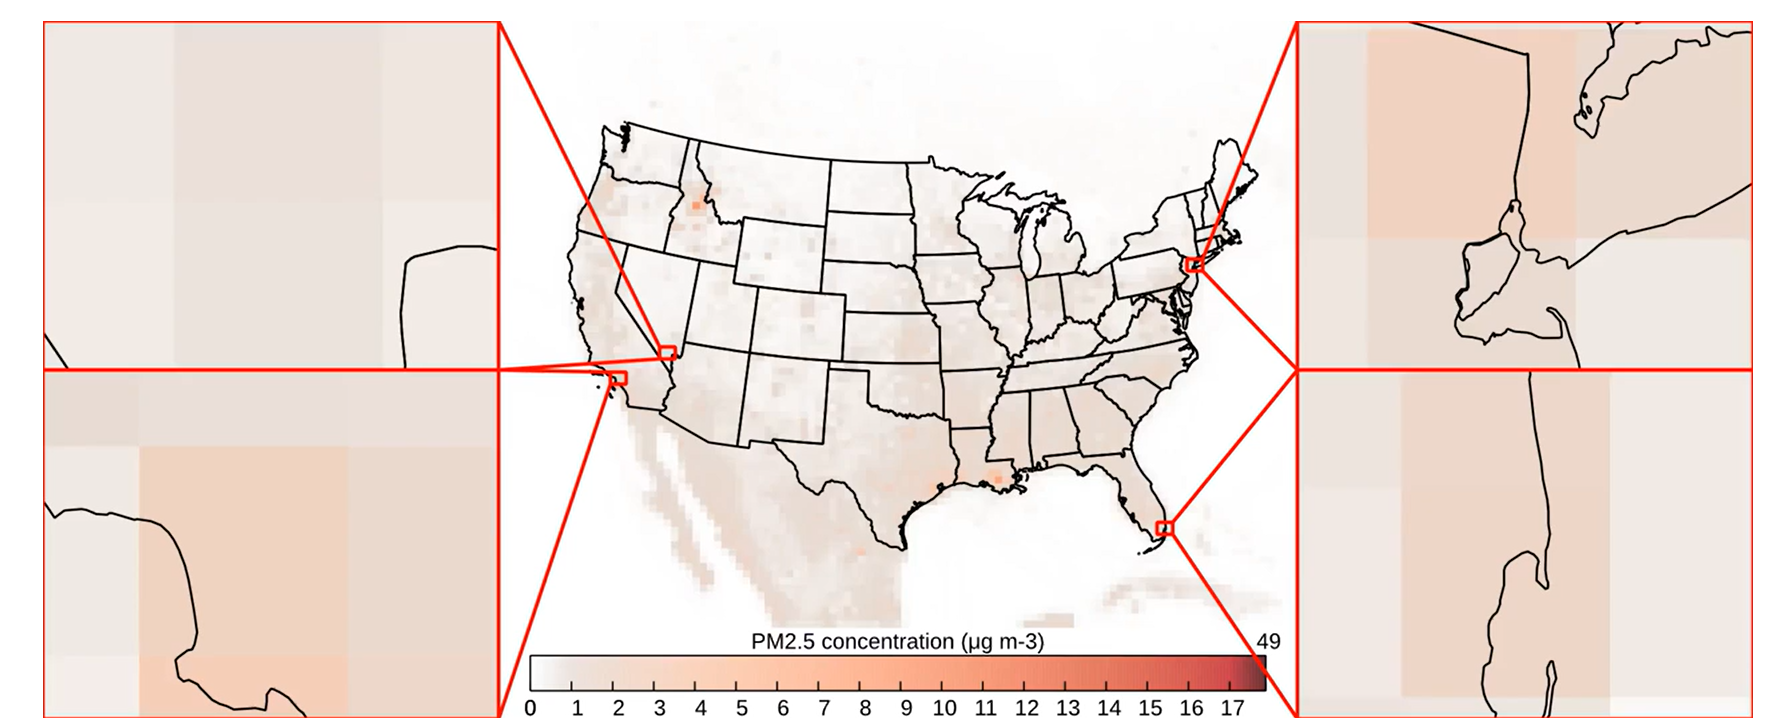
\includegraphics[width=0.8\textwidth]{inmap2.png}
    \caption{The result of the model when running with $\text{PM}_{2.5}$ as the specified pollutant.}
    \label{fig:grid2}
 \end{figure}

\end{document}
